\section{Datasets}
\label{section:Architecture:Dataset}

The complete dataset supplied by "Prisguiden.no" contains over 1300 unique product categories.
To achieve product trend predictions of categories the dataset is split into smaller subsets of data to be analyzed.
These datasets create the basis for the experiments to be conducted.
Initially, 4 datasets were selected, each with its own properties and connectivity.
The first two datasets are created based on correlation.
The first dataset is defined with 20 highly correlating categories, while the second is comprised of 20 categories with the least prediction.
This is done in order to evaluate the machine learning methods on whether or not predictions can be improved using correlating data.

Dataset 3 is comprised of seasonal data with high extreme values.
Lastly, dataset 4 is comprised of a set of completely random categories.


\subsection{Dataset 1 - Correlation}

% 1. Why is a correlating dataset selected? What is the aim?
A dataset with a high correlation between the categories is selected with the aim of using the correlation to improve the model predictions.
The hope is that the correlating data gives global models more relevant data to work with.
This can then be compared to a non-correlating dataset (dataset 2) in order to evaluate the importance of the data correlation in this case.

% 2. How was the search conducted? Manual search using domain knowledge!
In order to select correlating time series as part of the correlating dataset, a combination of manual data selection through domain knowledge and auto-correlation was used.
A method for calculating auto-correlation was used in order to create a heat map of correlation between all the categories.
Category autocorrelation was calculated using 
% TODO! Explain the auto-correlation settings 100 points
Using this heat map, we were able to evaluate what clusters of categories had the highest concentration of autocorrelation.
In order to make correlating datasets stand out more clearly, we remove values from category pairs with an auto-correlation lower than 0.5 across the categories. 
% Heatmap image of all categories
\begin{figure}[h!]
  \centering
  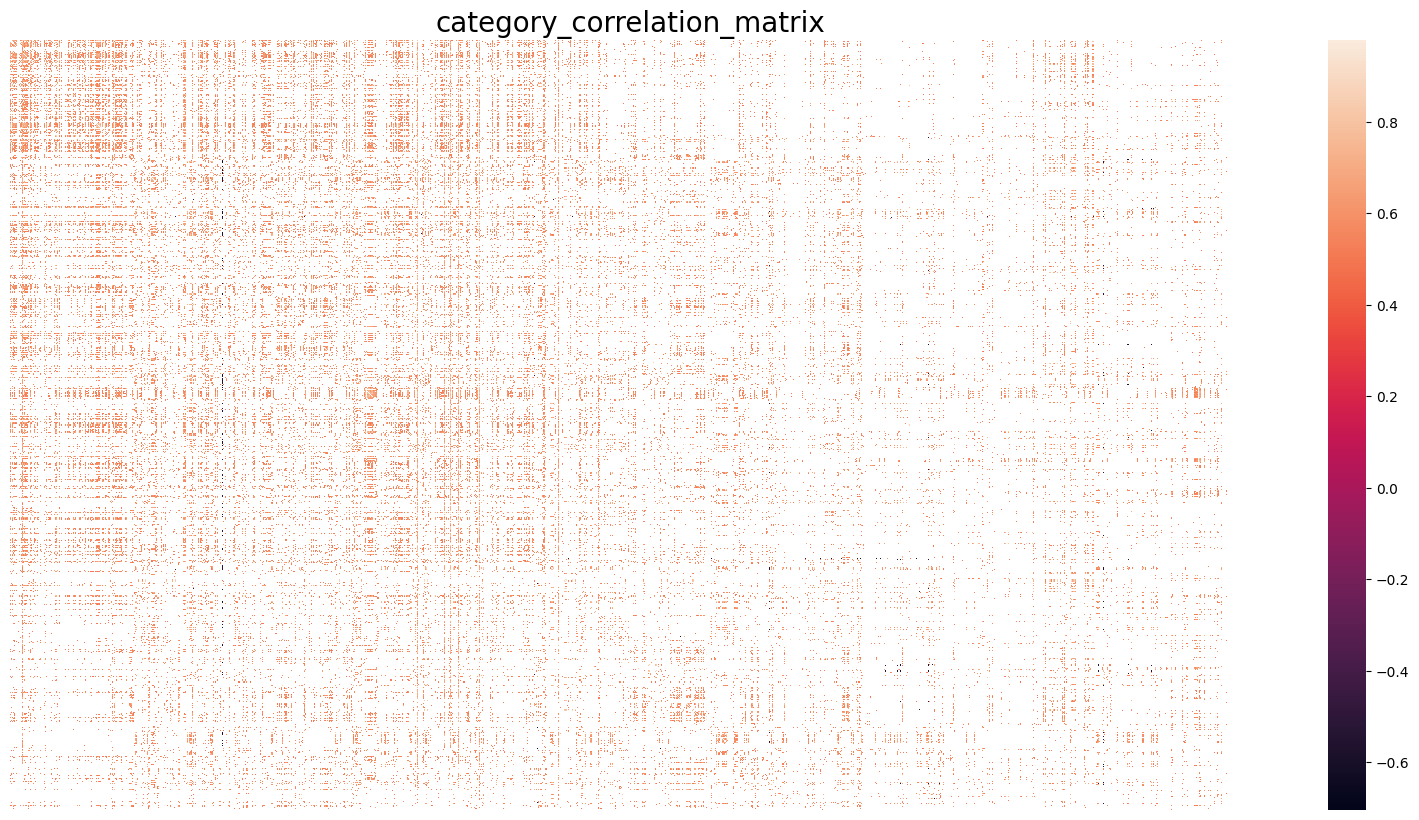
\includegraphics[width=\textwidth]{./figs/dataset/category_correlation_matrix.png}
  \hfill
  \caption{A correlation matrix showing the autocorrelation of all categories, filtered out values of autocorrelation below 0.5 in order to increase visibility of high correlation values and groupings.}
  \label{fig:dataset:heatmap_correlating}
\end{figure}

Using the heatmap as a reference, it was clear that the interval of the first 30 or so categories has a high autocorrelation.
Additionally, the categories with the highest correlation are all categories contained within the domain of electronics.
Using domain knowledge we are able to assert that these categories should have a higher correlation between them than other categories probably have.
With these two assumptions comprising the basis for the selection, we were able to filter out categories with less correlation, resulting in a set of 20 categories comprising the correlating dataset.
% Heatmap image of the selected 20 categories in the Correlation dataset
\begin{figure}[h!]
  \centering
  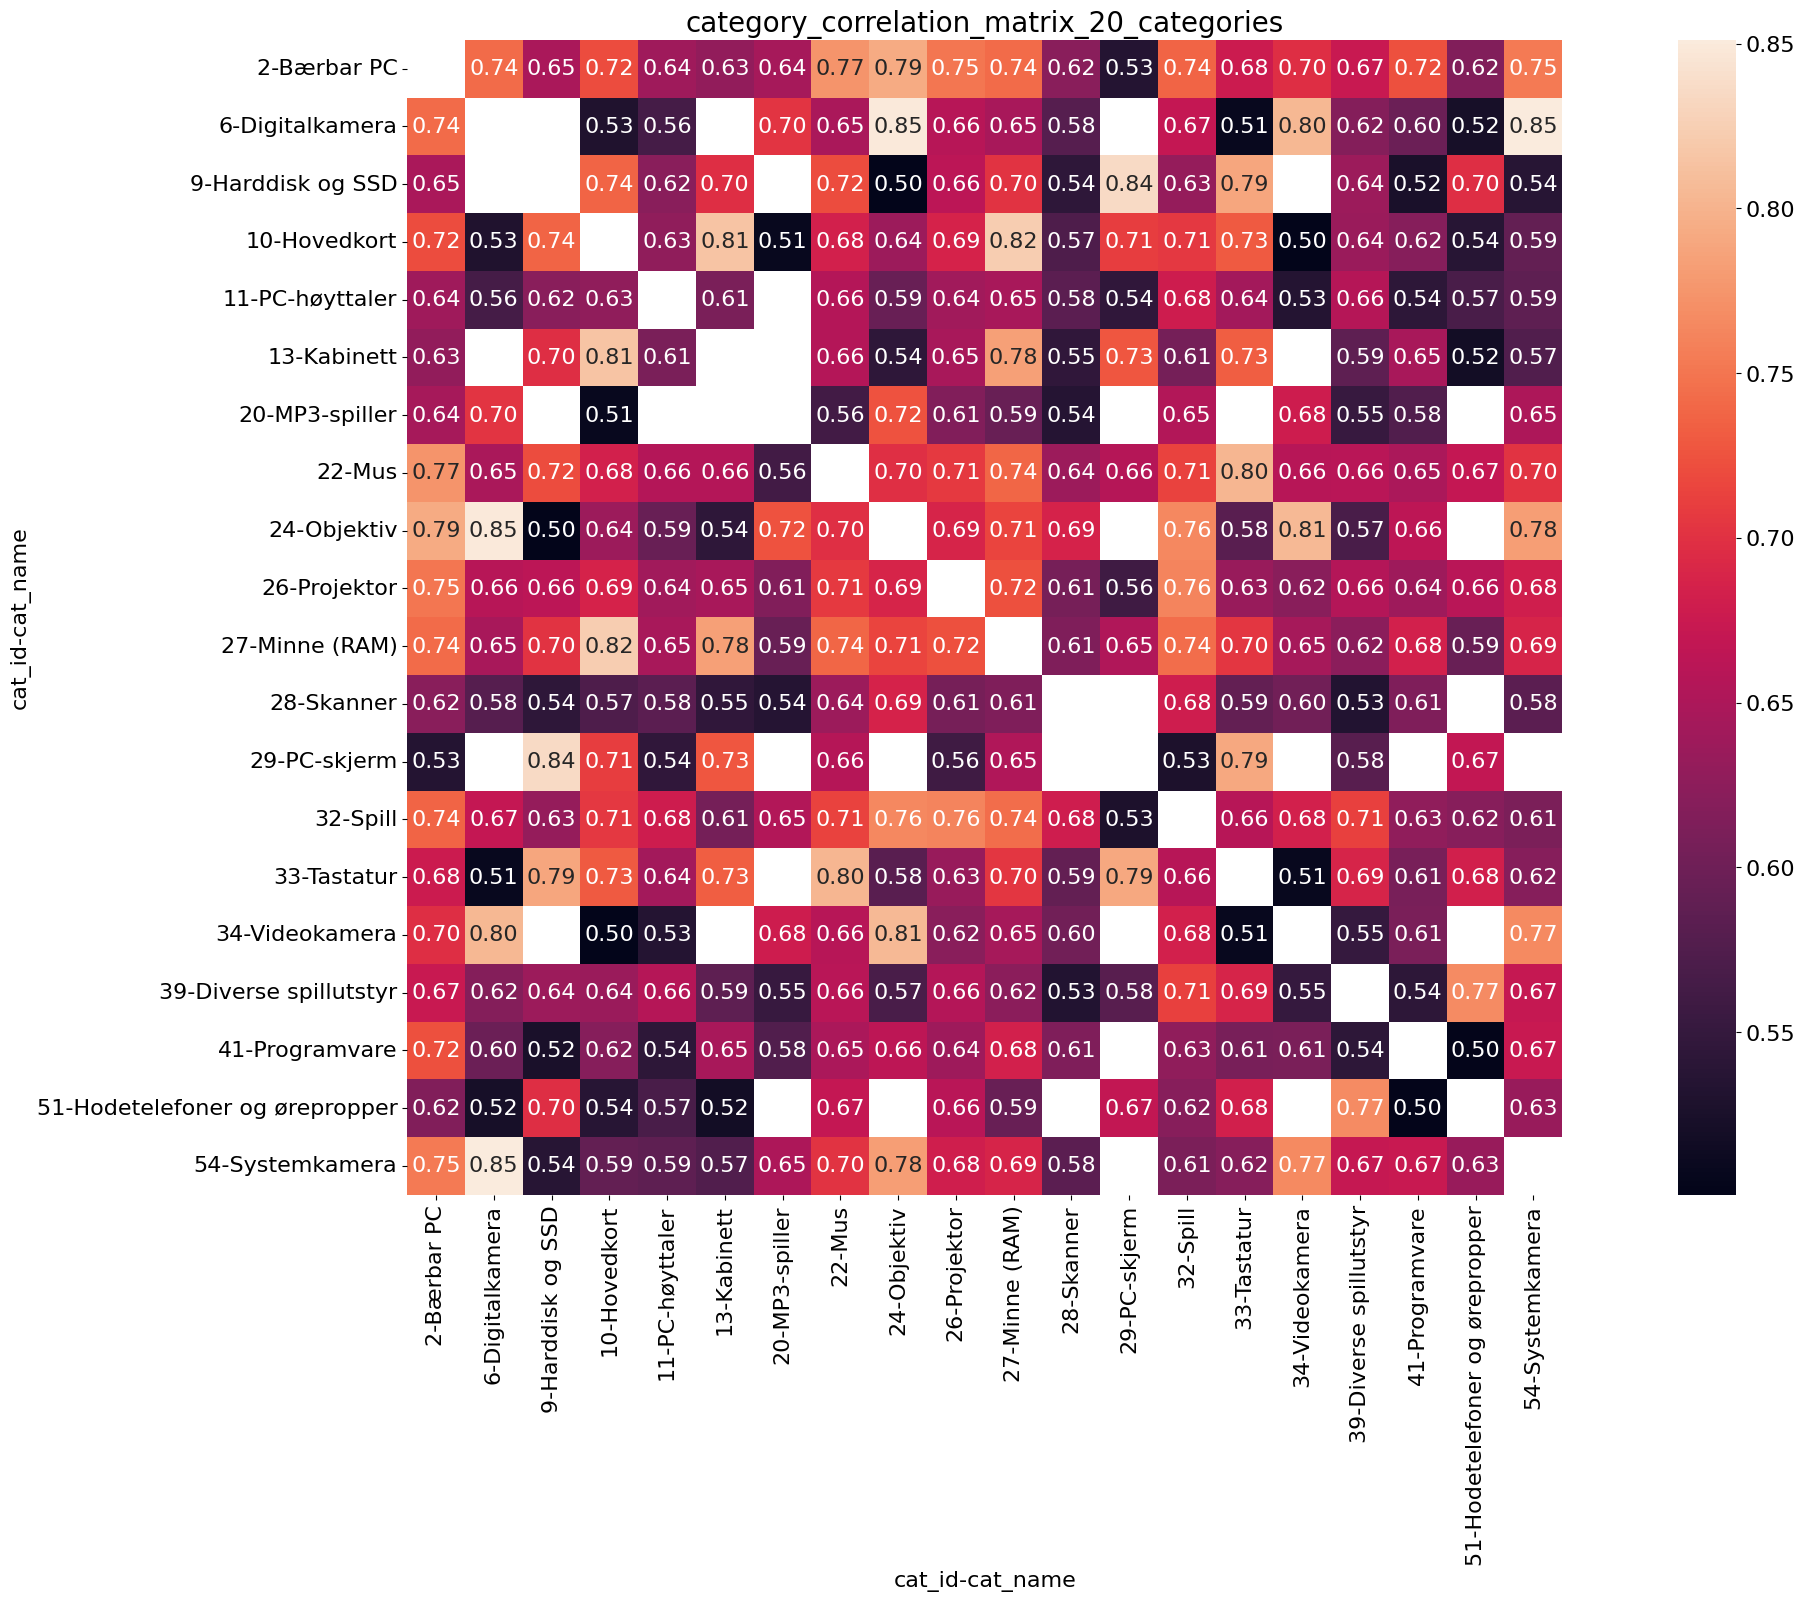
\includegraphics[width=\textwidth]{./figs/dataset/category_correlation_matrix_20_categories.png}
  \hfill
  \caption{A correlation matrix showing the autocorrelation between the selected 20 categories of the highly correlating category dataset - Dataset 1.}
  \label{fig:dataset:heatmap_20_correlating}
\end{figure}


% 3. What data was selected?
The filtered dataset contains 20 categories from the electronics domain, some of the most highly correlating datasets in our dataset.
The selected categories are:

% Insert list of categorie
\begin{table}[h]
  \centering
  \caption{Selected categories comprising dataset 1 - Correlating categories}
  \label{table:dataset1}
  \begin{tabular}{|c|l|l|}\hline
    Category ID & Name(Norwegian)    & Name(English)   \\ \hline
    2    & Bærbar PC              & TODO                 \\ \hline
    6    & Digitalkamera          & TODO                 \\ \hline
    9    & Harddisk og SSD        & TODO                 \\ \hline
    10   & Hovedkort              & TODO                 \\ \hline
    11   & PC-høytaler            & TODO                 \\ \hline
    13   & Kabinett               & TODO                 \\ \hline
    20   & MP3-Spiller            & TODO                 \\ \hline
    22   & Mus                    & TODO                 \\ \hline
    24   & Objektir               & TODO                 \\ \hline
    26   & Prosjektor             & TODO                 \\ \hline
    27   & Minne (RAM)            & TODO                 \\ \hline
    28   & Skanner                & TODO                 \\ \hline
    29   & PC-skjerm              & TODO                 \\ \hline
    32   & Spill                  & TODO                 \\ \hline
    33   & Tastatur               & TODO                 \\ \hline
    34   & Videokamera            & TODO                 \\ \hline
    39   & Diverse spillutstyr    & TODO                 \\ \hline
    41   & Programvare            & TODO                 \\ \hline
    51   & Hodetelefoner          & TODO                 \\ \hline
    54   & Systemkamera           & TODO                 \\ \hline
  \end{tabular}
\end{table}



\subsection{Dataset 2 - No Correlation}

% 1. Why is a no-corrolation dataset selected? What is the aim?
As the second dataset, a collection of 20 categories with the lowest possible correlation is defined.
A dataset with close to no natural correlation either through autocorrelation or through the use of domain knowledge, the second dataset is defined in order to serve as an opposite to the first dataset.
This dataset is meant to serve as an opposite to the first dataset, making it easier to evaluate if the correlation between categories has any significant effect on forecasting.

% 2. How was the search conducted? Sorted search, using manual tuning in the end.
To find a set of 20 categories with the lowest possible correlation, we conducted a search on the values of calculated auto-correlation.
Using auto-correlation analysis on the dataset, the categories were sorted after the amount of correlation summed across all categories.
Out of the sorted list, the top 50 categories with the least correlation were selected.
Of these 50, seasonal categories such as product categories related to Christmas were filtered out.
After this, a manual selection was conducted on the remaining categories in order to remove those with a high correlation between the remaining categories.
This was repeated until only 20 categories remain.
% Insert image of the 20 non correlating categories
\begin{figure}[h!]
  \centering
  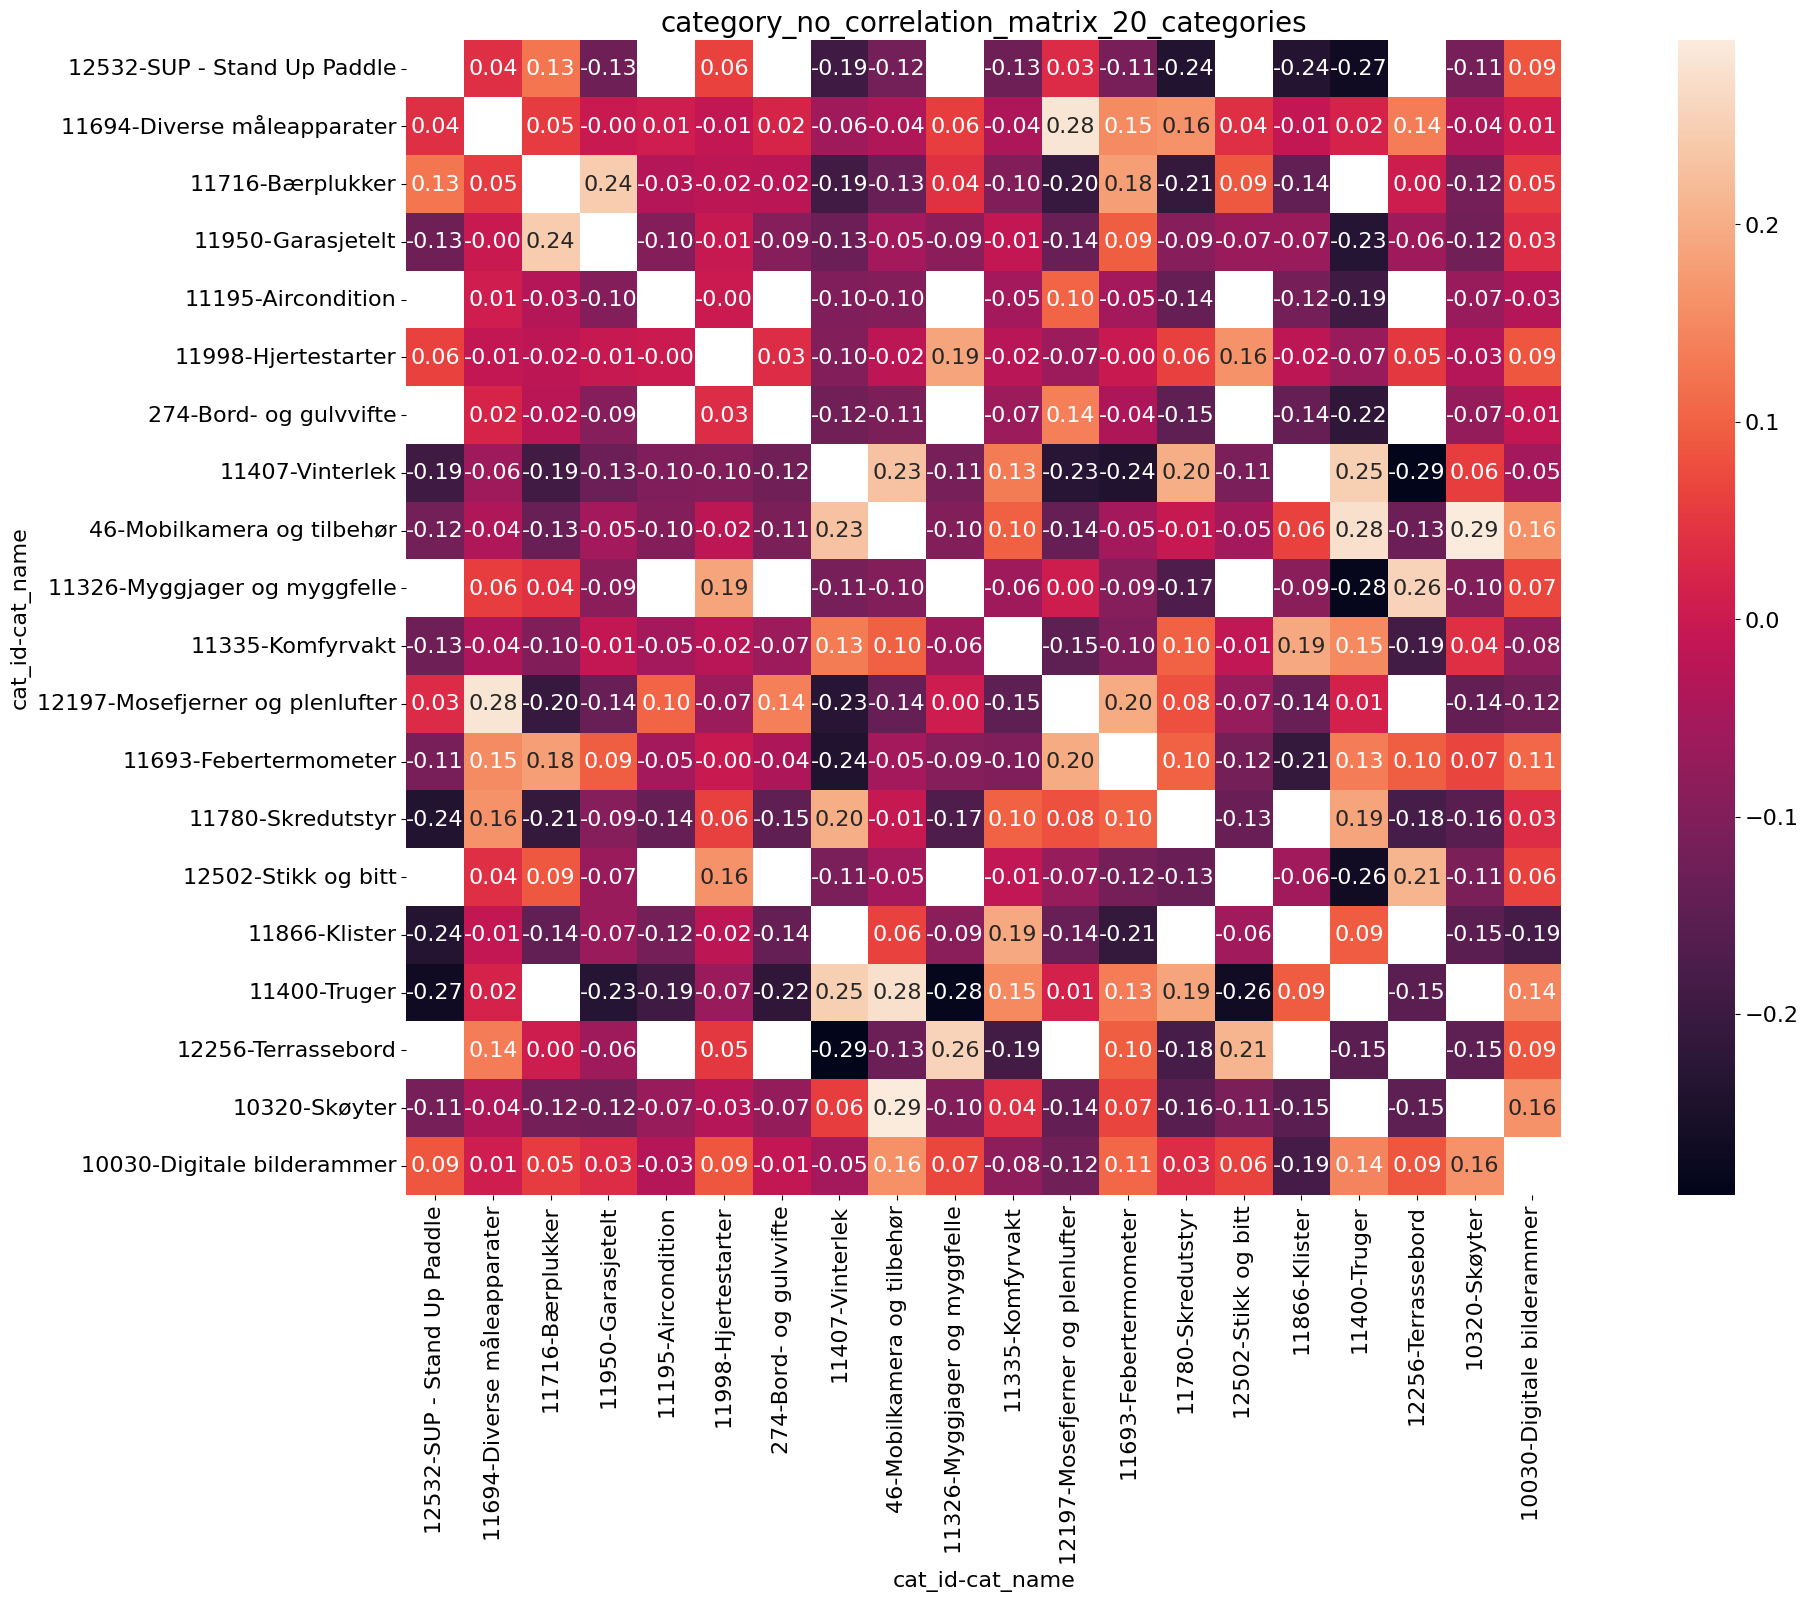
\includegraphics[width=\textwidth]{./figs/dataset/category_no_correlation_matrix_20_categories.png}
  \hfill
  \caption{A correlation matrix showing the autocorrelation between the selected 20 categories with the lowest autocorrelation - Dataset 2.}
  \label{fig:dataset:heatmap_20_no_correlating}
\end{figure}



% 3. What data was selected? <Image>
The filtered dataset contains 20 categories with the least inward correlation we could find.
The selected categories are:

\begin{table}[h]
  \centering
  \caption{Selected categories comprising dataset 1 - Correlating categories}
  \label{table:dataset1}
  \begin{tabular}{|c|l|l|}\hline
    Category ID & Name(Norwegian)             & Name(English)   \\ \hline
    12532   & Hodetelefoner                   & TODO                 \\ \hline
    11694   & Diverse måleapparater           & TODO                 \\ \hline
    11716   & Bærplukker                      & TODO                 \\ \hline
    11950   & Garasjetelt                     & TODO                 \\ \hline
    11988   & Aircondition                    & TODO                 \\ \hline
    11998   & Hjertestarter                   & TODO                 \\ \hline
    274     & Bord- og gulvvifte              & TODO                 \\ \hline
    11407   & Vinterlek                       & TODO                 \\ \hline
    46      & Mobilkamera og tilbehør         & TODO                 \\ \hline
    11326   & Myggjager og myggfelle          & TODO                 \\ \hline
    11335   & Komfyrvakt                      & TODO                 \\ \hline
    12197   & Mosefjerner og plenlufter       & TODO                 \\ \hline
    11693   & Febertermometer                 & TODO                 \\ \hline
    11780   & Skredutstyr                     & TODO                 \\ \hline
    12502   & Stikk og bitt                   & TODO                 \\ \hline
    11866   & Klister                         & TODO                 \\ \hline
    11400   & Truger                          & TODO                 \\ \hline
    12256   & Terrassebord                    & TODO                 \\ \hline
    10320   & Skøyter                         & TODO                 \\ \hline
    10030   & Digitale bilderammer            & TODO                 \\ \hline
  \end{tabular}
\end{table}


\subsection{Dataset 3 - }
% TODO!
\textbf{TODO}

\subsection{Dataset 4 - }
% TODO!
\textbf{TODO}
